\section{Auswertung}
\label{sec:Auswertung}
\begin{figure}
  \centering
  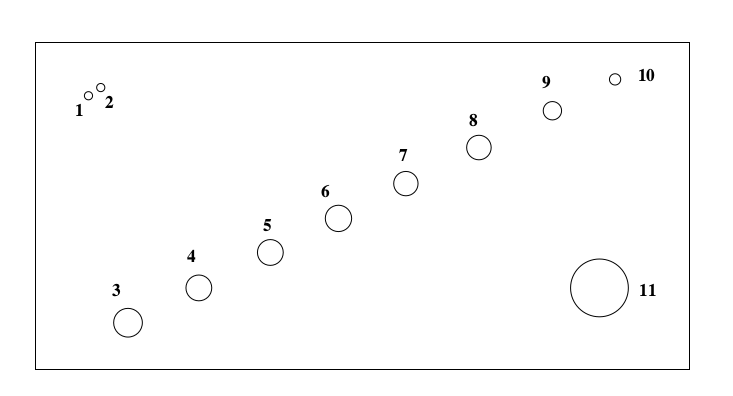
\includegraphics[width=0.8\textwidth]{Bilder/fehlstellen.png}
  \caption{Schematische Darstellung des untersuchten Acrylblocks samt der durchnummerierten Fehlstellen. \cite{Anleitung}.}
  \label{fig:fehlstellen}
\end{figure}
Zunächst werden die Durchmesser $d$ sämtlicher Fehlstellen mittels einer Schiebelehre ausgemessen. Die Nummerierung $n$ der Fehlstellen erfolgt nach dem Schema in Abbildung \ref{fig:fehlstellen}. Die bestimmten Durchmesser finden sich in Tabelle \ref{tab:fehlstellen}.
\begin{table}
  \centering
	\caption{Durchmesser der Fehlstellen vermessen mittels Schieblehre.}
	\label{tab:fehlstellen}
	\begin{tabular}{cc}
		\toprule
    $n$ & $d$/$\si{\milli\meter}$ \\
		\midrule
1.0 & 1.3 \\
2.0 & 1.3 \\
3.0 & 5.8 \\
4.0 & 4.8 \\
5.0 & 4.0 \\
6.0 & 2.9 \\
7.0 & 2.9 \\
8.0 & 2.9 \\
9.0 & 2.9 \\
10.0 & 2.9 \\
11.0 & 9.5 \\
\bottomrule
\end{tabular}
\end{table}
Zusätzlich wurde der gesamte Acrylblock mittels der Schiebelehre vermessen. Es ergibt sich eine Breite von ${\SI{8}{\centi\meter}}$. Mit der Schallgeschwindigkeit ${c=\SI{2730}{\meter\per\second}}$ nach \cite{schall} und Formel \eqref{eqn:laufzeit} ergibt sich die Laufzeit des Ultraschallsignals durch den Acrylblock zu ${t_{\mathrm{theo}}=\SI{58.6}{\micro\second}}$.
Wird allerdings die tatsächliche Laufzeit des Ultraschallsignals in der Messung bestimmt, ergibt sich eine Laufzeit von ${t_\mathrm{real}=\SI{60.6}{\micro\second}}$. Dies liegt an der Anpassungsschicht zwischen der Ultraschallsonde und dem Acrylblock. Um in den weiteren Messungen die tatsächlichen Laufzeiten im Acrylblock zu bestimmen, muss von jedem bestimmten Wert daher die Laufzeit durch die Anpassungsschicht ${\Delta t=\SI{2}{\micro\second}}$ abgezogen werden.











%%%%%%%%%%%%%%%%%%%%%%BScan%%%%%%%%%%%%%%%%%%%%%%%%%
\subsection{Bestimmung der Abmessung der Fehlstellen über den B-Scan.}
Zur Bestimmung der Abmessung der Fehlstellen über den B-Scan wird die Lage jeder Fehlstelle mittels des freien Grafikprogramms \enquote{gimp}











%%Vorlagen
%Bild
%\begin{figure}
%  \centering
%  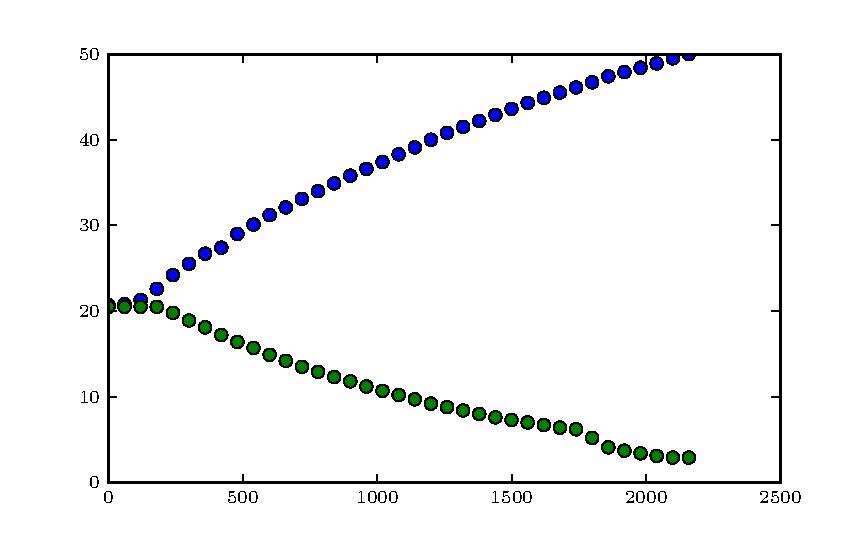
\includegraphics{plot.pdf}
%  \caption{Plot.}
%  \label{fig:plot}
%\end{figure}


%Tabelle
%\begin{table}
%	\centering
%	\caption{Table.}
%	\label{tab:table}
%	\begin{tabular}{ccc}
%		\toprule
%    column1&column2&column3\\
%		\midrule
%		220 & -391 & 659 \\
%		330 & -598 & 946 \\
%		525 & -1000 & 1660 \\
%		702 & -1337 & 2051 \\
%		930 & -1650 & 2450 \\
%		\bottomrule
%	\end{tabular}
%\end{table}
